\subsection{Query Processing}

\textbf{Query Processing} (Xử lý truy vấn) là quá trình chuyển đổi câu lệnh truy vấn do người dùng nhập (ví dụ: SQL trong các cơ sở dữ liệu quan hệ hay MQL trong MongoDB) thành một kế hoạch thực thi hiệu quả để truy xuất dữ liệu từ cơ sở dữ liệu. 

\textbf{Query processing} (xử lý truy vấn) là một quy trình phức tạp trong hệ thống cơ sở dữ liệu, bao gồm các bước từ khi nhận truy vấn từ người dùng đến khi trả về kết quả. Quy trình này đóng vai trò then chốt, quyết định hiệu suất và độ tin cậy của hệ thống cơ sở dữ liệu.

\textbf{Query processing} là chuỗi các hoạt động xử lý truy vấn trong hệ thống cơ sở dữ liệu, bao gồm:

\begin{itemize}
    \item Phân tích cú pháp truy vấn
    \item Kiểm tra tính hợp lệ
    \item Tối ưu hóa truy vấn
    \item Tạo kế hoạch thực thi
    \item Thực thi truy vấn
    \item Tổng hợp và trả về kết quả
\end{itemize}

\noindent
\textbf{Vai trò và Lợi ích của Query Processing}

\begin{itemize}
    \item Tăng hiệu năng truy xuất dữ liệu:
    \begin{itemize}
        \item Giúp giảm thiểu thời gian truy vấn thông qua tối ưu hóa kế hoạch thực thi.
    \end{itemize}
    \item Quản lý tài nguyên hiệu quả:
    \begin{itemize}
        \item Giúp hệ thống sử dụng CPU, bộ nhớ và I/O một cách hợp lý, tránh việc quét toàn bộ bảng không cần thiết.
    \end{itemize}
    \item Hỗ trợ truy vấn phức tạp:
    \begin{itemize}
        \item Cho phép xử lý các truy vấn có nhiều phép toán như join, subquery, aggregate… một cách hiệu quả.
    \end{itemize}
\end{itemize}

\textbf{Query Processing} đóng vai trò quan trọng trong việc đảm bảo rằng hệ thống cơ sở dữ liệu thực thi các truy vấn một cách nhanh chóng và hiệu quả, góp phần nâng cao hiệu năng tổng thể của ứng dụng.

\newpage

\subsubsection{Postgres}

PostgreSQL là một hệ quản trị cơ sở dữ liệu quan hệ mã nguồn mở với kiến trúc xử lý truy vấn phức tạp và hiệu quả.

Dưới đây là mô hình hoạt động của query processing trong PostgreSQL:

\begin{tikzpicture}[node distance=0.5cm and 0.5cm, auto,
    block/.style={rectangle, draw, text centered, rounded corners},
    line/.style={draw, -Latex}]

  % Main flow nodes
  \node (sql) [block] {SQL Query};
  \node (parser) [block, right=of sql] {Parser};
  \node (analyzer) [block, right=of parser] {Analyzer};
  \node (rewriter) [block, right=of analyzer] {Rewriter};
  \node (optimizer) [block, right=of rewriter] {Planner/Optimizer};
  \node (executor) [block, right=of optimizer] {Executor};
  \node (results) [block, right=of executor] {Results};

  % Feedback loop nodes
  \node (catalog) [block, below=1.5cm of analyzer] {Catalog};
  \node (rules) [block, below=1.5cm of rewriter] {Rule System};
  \node (stats) [block, below=1.5cm of optimizer] {Statistics};

  % Arrows for the main flow
  \draw [line] (sql) -- (parser);
  \draw [line] (parser) -- (analyzer);
  \draw [line] (analyzer) -- (rewriter);
  \draw [line] (rewriter) -- (optimizer);
  \draw [line] (optimizer) -- (executor);
  \draw [line] (executor) -- (results);

  % Arrows for the feedback loops
  \draw [line] (rules) -- (rewriter);
  \draw [line] (catalog) -- (analyzer); % Feedback to Analyzer
  \draw [line] (stats) -- (optimizer); % Feedback to Optimizer

\end{tikzpicture}


Quá trình này bao gồm một số bước chính:

\begin{enumerate}
    \item \textbf{Parser (Bộ phân tích cú pháp)}:
    \begin{itemize}
        \item Phân tích câu truy vấn để kiểm tra tính hợp lệ về cú pháp và đảm bảo rằng các từ khóa, tên bảng, tên trường, … được viết đúng theo quy tắc của ngôn ngữ truy vấn.
        \item Trình phân tích cú pháp truy vấn phân tích cấu trúc cú pháp của truy vấn, đảm bảo nó tuân thủ các quy tắc ngữ pháp của ngôn ngữ PostgreSQL. Nó kiểm tra lỗi, xác thực cấu trúc truy vấn và tạo cây phân tích cú pháp. Đầu ra là một cây phân tích cú pháp : 

      \begin{figure}[H]
                    \centering
                    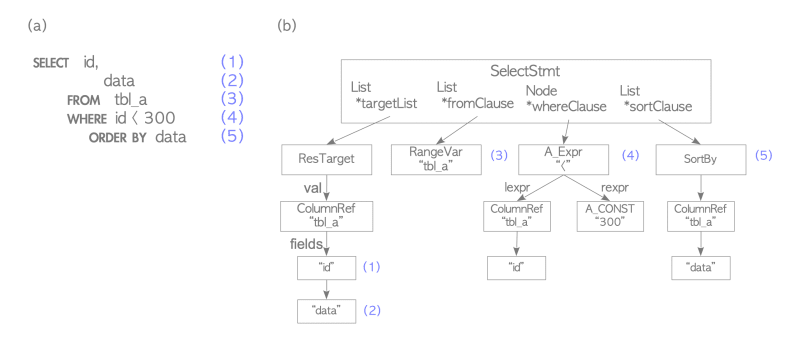
\includegraphics[width = 1\textwidth]{Images/query-progress-01.png}
                    \caption{Ví dụ cây phân tích cú pháp}
                \end{figure}
                
    \end{itemize}
     \item \textbf{Semantic Analysis}:
    \begin{itemize}
        \item  Sau khi phân tích cú pháp thành công, trình phân tích ngữ nghĩa (semantic analyzer) sẽ kiểm tra ý nghĩa của câu truy vấn. Nó xác minh sự tồn tại của các bảng, cột, hàm và các đối tượng cơ sở dữ liệu khác được tham chiếu trong truy vấn. Nó cũng kiểm tra quyền truy cập của người dùng để đảm bảo họ có quyền thực hiện truy vấn.
        \item Kiểm tra tính hợp lệ của truy vấn
        \item Xác minh rằng các bảng, cột và hàm được tham chiếu tồn tại
        \item Phân giải các tên cột và kiểm tra quyền truy cập
        \item Chuyển đổi parse tree thành query tree
        \item Xác định kiểu dữ liệu cho mỗi biểu thức
    \end{itemize}
    \item \textbf{Query Rewriting (Chuyển đổi truy vấn)}:
    \begin{itemize}
        \item Giai đoạn này có thể xảy ra nếu có các quy tắc (rules) hoặc view được định nghĩa. Trình viết lại (rewriter) có thể sửa đổi câu truy vấn ban đầu dựa trên các quy tắc này để tối ưu hóa hoặc thực hiện các logic phức tạp.
        \item Biến đổi câu truy vấn ban đầu thành dạng dễ tối ưu hóa hơn, chẳng hạn như đơn giản hóa các biểu thức logic hoặc chuyển đổi cấu trúc của câu truy vấn.
        \item Áp dụng các quy tắc từ hệ thống rules
        \item Mở rộng view thành các truy vấn trên bảng cơ sở
        \item Áp dụng các ràng buộc bảo mật (Row-Level Security)
        \item Xử lý các trigger và policy
    \end{itemize}
    \item \textbf{Planner/Optimizer (Bộ lập kế hoạch/tối ưu hóa)}:
    \begin{itemize}
        \item Đây là giai đoạn quan trọng nhất. Trình lập kế hoạch (planner) sẽ tạo ra nhiều kế hoạch thực thi khác nhau cho cùng một câu truy vấn. Mỗi kế hoạch này bao gồm các bước cụ thể để truy cập và xử lý dữ liệu, chẳng hạn như sử dụng index, thực hiện sequential scan, hoặc chọn thuật toán join phù hợp.
        \item PostgreSQL sẽ tạo kế hoạch thực thi (execution plan) bằng cách chọn phương án tối ưu nhất dựa trên các chỉ mục và thống kê dữ liệu. Điều này bao gồm việc quyết định thứ tự thực thi các bước trong truy vấn.
        \item Xác định kế hoạch thực thi tối ưu bằng cách cân nhắc nhiều phương án khác nhau. Hệ quản trị cơ sở dữ liệu sẽ dựa vào các thống kê dữ liệu, cấu trúc bảng, chỉ mục, … để lựa chọn chiến lược tốt nhất nhằm giảm thiểu thời gian và tài nguyên cần thiết cho truy vấn.
        \item Trình tối ưu hóa (optimizer) sẽ đánh giá chi phí ước tính của mỗi kế hoạch thực thi được tạo ra bởi trình lập kế hoạch. Chi phí này thường được tính toán dựa trên các yếu tố như thời gian thực thi dự kiến, số lượng I/O cần thiết và mức sử dụng tài nguyên hệ thống. Trình tối ưu hóa sẽ chọn kế hoạch có chi phí thấp nhất để thực thi.
        \item Phân tích nhiều kế hoạch thực thi có thể
        \item Ước tính chi phí cho mỗi kế hoạch dựa trên thống kê
        \item Lựa chọn kế hoạch có chi phí thấp nhất
        \item Xác định chiến lược quét (table scan, index scan)
        \item Quyết định phương pháp join (nested loop, hash join, merge join)
        \item Tối ưu hóa các phép lọc và sắp xếp
    \end{itemize}
    \item \textbf{Query Execution (Thực thi truy vấn)}:
    \begin{itemize}
        \item Thực hiện kế hoạch truy vấn đã được tối ưu hóa, truy xuất dữ liệu từ các bảng hoặc collections theo cách hiệu quả nhất.
    \end{itemize}
    \item \textbf{Formatting (Định dạng kết quả)}:
    \begin{itemize}
        \item Sau khi truy xuất dữ liệu, kết quả được định dạng lại và trả về cho người dùng hoặc ứng dụng theo yêu cầu.
    \end{itemize}
\end{enumerate}

\textbf{Đặc điểm} : 
\begin{itemize}
    \item Sử dụng SQL, hỗ trợ  các truy vấn phức tạp như join, subquery, aggregate.
    \item Có query optimizer mạnh mẽ giúp tối ưu thời gian thực thi.
\end{itemize}

\textbf{Ví dụ Code (SQL)}:

\begin{lstlisting}[style=sql, caption=Ví dụ query trong Postgres, label=sql:example]
SELECT u.name, o.order_date
FROM users u
JOIN orders o ON u.id = o.user_id
WHERE u.email = 'john.doe@example.com';
\end{lstlisting}


\textbf{Query Optimization trong PostgreSQL}

\textbf{Query optimization} trong PostgreSQL là quá trình tự động hoặc thủ công để cải thiện hiệu suất của các câu truy vấn SQL. Mục tiêu là giảm thiểu thời gian thực thi và tài nguyên hệ thống cần thiết.

Có nhiều kỹ thuật để tối ưu hóa truy vấn trong PostgreSQL:

\begin{enumerate}
    \item \textbf{Sử dụng Index}: Index là cấu trúc dữ liệu đặc biệt giúp PostgreSQL tìm kiếm các hàng cụ thể trong bảng một cách nhanh chóng. Tạo index trên các cột thường xuyên được sử dụng trong mệnh đề \textbf{WHERE}, \textbf{JOIN}, \textbf{ORDER BY}, và \textbf{GROUP BY}.
    \begin{itemize}
        \item \textbf{Index Optimization}: Sử dụng B-tree, Hash, GIN, GiST.
        \begin{itemize}
            \item \textbf{B-tree indexes}: Chỉ mục chuẩn cho các phép so sánh =, <, >, <=, >=:     
\begin{lstlisting}[style=sql, caption=Ví dụ sử dụng B-tree indexes trong Postgres, label=sql:example]
CREATE INDEX idx\_employee\_name ON employees(name);
\end{lstlisting}
            \item \textbf{Hash indexes} : Hiệu quả cho phép so sánh bằng.
\begin{lstlisting}[style=sql, caption=Ví dụ sử dụng Hash indexes trong Postgres, label=sql:example]
CREATE INDEX idx_employee_id_hash ON employees USING HASH (employee_id);
\end{lstlisting}
            \item \textbf{GiST indexes}: Cho dữ liệu không chuẩn (hình học, văn bản)
\begin{lstlisting}[style=sql, caption=Ví dụ sử dụng Hash indexes trong Postgres, label=sql:example]
CREATE INDEX idx_location ON stores USING GIST (location);
\end{lstlisting}
            \item \textbf{GIN indexes}: Cho dữ liệu có nhiều giá trị trong một trường (arrays, jsonb)
\begin{lstlisting}[style=sql, caption=Ví dụ sử dụng GIN indexes trong Postgres, label=sql:example]
CREATE INDEX idx_tags ON products USING GIN (tags);
\end{lstlisting}

            \item \textbf{BRIN indexes}: Cho dữ liệu có tổ chức tự nhiên (timestamps)
\begin{lstlisting}[style=sql, caption=Ví dụ sử dụng BRIN indexes trong Postgres, label=sql:example]
CREATE INDEX idx_timestamp ON logs USING BRIN (created_at);
\end{lstlisting}

            \item \textbf{Partial indexes}: Chỉ đánh chỉ mục cho một phần dữ liệu
\begin{lstlisting}[style=sql, caption=Ví dụ sử dụng Partial indexes trong Postgres, label=sql:example]
CREATE INDEX idx_active_users ON users(email) WHERE status = 'active';
\end{lstlisting}

            \item \textbf{Multi-column indexes}: Đánh chỉ mục nhiều cột
\begin{lstlisting}[style=sql, caption=Ví dụ sử dụng Multi-column indexes trong Postgres, label=sql:example]
CREATE INDEX idx_name_dept ON employees(department_id, last_name, first_name);
\end{lstlisting}
        \end{itemize}
        \item \textbf{Join Ordering}: Chọn thứ tự join tối ưu.

\begin{itemize}
    \item Chọn thứ tự join tối ưu
    \item Lựa chọn phương pháp join phù hợp (nested loop, hash, merge)
    \item Sử dụng join column indexes
    \item Tận dụng foreign keys
\end{itemize}

        \item \textbf{Parallel Query}: Thực thi song song.
        \item \textbf{WHERE Clause Optimization}

\begin{itemize}
    \item Sử dụng điều kiện có thể tận dụng các chỉ mục
    \item Tránh sử dụng các hàm trên cột được lọc
    \item Tận dụng phép lọc có độ chọn lọc cao
    \item Sử dụng điều kiện IN thay vì nhiều điều kiện OR
\end{itemize}

\begin{lstlisting}[style=sql, caption=Ví dụ tối ưu WHERE Clause Optimization trong Postgres, label=sql:example]
-- Tốt
SELECT * FROM orders WHERE status IN ('pending', 'processing');

-- Kém hiệu quả
SELECT * FROM orders WHERE status = 'pending' OR status = 'processing';
\end{lstlisting}


        \item \textbf{Partition Pruning}:


\begin{itemize}
    \item Chia dữ liệu thành các phân vùng
    \item Chỉ quét các phân vùng liên quan
\end{itemize}

\begin{lstlisting}[style=sql, caption=Ví dụ Partition Pruning trong Postgres, label=sql:example]
CREATE TABLE sales (
    id SERIAL,
    sale_date DATE,
    amount NUMERIC
) PARTITION BY RANGE (sale_date);

CREATE TABLE sales_2023 PARTITION OF sales
    FOR VALUES FROM ('2023-01-01') TO ('2024-01-01');

CREATE TABLE sales_2024 PARTITION OF sales
    FOR VALUES FROM ('2024-01-01') TO ('2025-01-01');
\end{lstlisting}        
        
        \item \textbf{Materialized Views}: Lưu kết quả truy vấn thường dùng.

\begin{lstlisting}[style=sql, caption=Ví dụ Materialized Views trong Postgres, label=sql:example]
CREATE MATERIALIZED VIEW sales_summary AS
SELECT 
    date_trunc('month', sale_date) AS month,
    product_id,
    SUM(quantity) AS total_quantity,
    SUM(amount) AS total_amount
FROM sales
GROUP BY date_trunc('month', sale_date), product_id;

REFRESH MATERIALIZED VIEW sales_summary;
\end{lstlisting}   

    \end{itemize}
    
    \item \textbf{Phân tích Kế hoạch Thực thi với \textit{EXPLAIN}}: Lệnh \textbf{EXPLAIN} cho phép bạn xem kế hoạch thực thi mà PostgreSQL sẽ sử dụng cho một câu truy vấn cụ thể. Điều này giúp bạn hiểu cách PostgreSQL truy cập dữ liệu và xác định các bước có thể được tối ưu hóa. Sử dụng \textbf{EXPLAIN\_ANALYZE} để có thông tin chi tiết về thời gian thực tế của từng bước.
\begin{lstlisting}[style=sql, caption=Ví dụ sử dụng EXPLAIN trong Postgres, label=sql:example]
EXPLAIN SELECT * FROM orders WHERE order_date > '2024-01-01';
EXPLAIN ANALYZE SELECT * FROM employees 
JOIN departments ON employees.department_id = departments.id
WHERE salary > 50000;


Nested Loop  (cost=0.29..34.38 rows=11 width=242) (actual time=0.038..0.078 rows=10 loops=1)
  ->  Index Scan using employees_department_id_idx on employees  (cost=0.29..16.79 rows=11 width=122) (actual time=0.020..0.033 rows=10 loops=1)
        Filter: (salary > 50000)
  ->  Index Scan using departments_pkey on departments  (cost=0.14..1.59 rows=1 width=120) (actual time=0.003..0.003 rows=1 loops=10)
        Index Cond: (id = employees.department_id)
Planning Time: 0.362 ms
Execution Time: 0.112 ms
\end{lstlisting}
    \item \textbf{Viết Truy vấn Hiệu quả}:
      \begin{itemize}
        \item Đơn giản hóa biểu thức phức tạp
        \item Loại bỏ các subqueries không cần thiết
        \item Chuyển đổi HAVING thành WHERE khi có thể
        \item Tối ưu hóa các phép UNION, INTERSECT và EXCEPT
        \item \textbf{Chỉ chọn các cột cần thiết}: Sử dụng \textbf{SELECT column1, column2} thay vì \textbf{SELECT *}.
        \item \textbf{Sử dụng mệnh đề \textit{WHERE} hiệu quả}: Lọc dữ liệu càng sớm càng tốt.
        \item \textbf{Tránh sử dụng các hàm trên các cột đã được index trong mệnh đề \textit{WHERE}}: Điều này có thể ngăn PostgreSQL sử dụng index. Thay vào đó, hãy xem xét tạo \textbf{functional index}.
        \item \textbf{Tối ưu hóa các phép toán \textit{JOIN}}: Hiểu rõ các loại \textbf{JOIN} và sử dụng loại phù hợp. Đảm bảo các cột tham gia trong \textbf{JOIN} được index.
        \item \textbf{Hạn chế sử dụng \textit{DISTINCT}}: Nếu có thể, hãy tìm cách khác để loại bỏ các bản ghi trùng lặp.
        \item \textbf{Sử dụng \textit{LIMIT}}: Nếu bạn chỉ cần một số lượng bản ghi nhất định, hãy sử dụng \textbf{LIMIT}.
    \end{itemize}
    \item \textbf{Cập nhật Thống kê với \textit{ANALYZE}}: PostgreSQL sử dụng thống kê về dữ liệu để đưa ra các quyết định tối ưu hóa. Chạy lệnh \textbf{ANALYZE} định kỳ trên các bảng để cập nhật thống kê.
\begin{lstlisting}[style=sql, caption=Ví dụ sử dụng ANALYZE trong Postgres, label=sql:example]
ANALYZE customers;
\end{lstlisting}

    \item \textbf{pg\_stat\_statements} : Theo dõi thống kê thực thi truy vấn

\begin{lstlisting}[style=sql, caption=Ví dụ theo dõi thống kê thực thi trong Postgres, label=sql:example]
SELECT query, calls, total_exec_time, rows, mean_exec_time
FROM pg_stat_statements
ORDER BY total_exec_time DESC
LIMIT 10;
\end{lstlisting}

    \item \textbf{auto\_explain} : Tự động ghi lại kế hoạch thực thi của các truy vấn chậm

\begin{lstlisting}[style=sql, caption=Ví dụ theo dõi truy vấn chậm trong Postgres, label=sql:example]
LOAD 'auto_explain';
SET auto_explain.log_min_duration = '100ms';
SET auto_explain.log_analyze = true;
\end{lstlisting}

    
    
    \item \textbf{Tối ưu hóa Cấu trúc Bảng}: Thiết kế bảng với các kiểu dữ liệu phù hợp và cân nhắc việc phân vùng bảng cho các bảng lớn.
    \item \textbf{Cấu hình PostgreSQL}: Điều chỉnh các tham số cấu hình như \textbf{shared\_buffers}, \textbf{work\_mem} có thể ảnh hưởng đến hiệu suất truy vấn.

    \begin{itemize}
        \item shared\_buffers: 25\% của RAM hệ thống
        \item effective\_cache\_size: 75\% của RAM hệ thống
        \item work\_mem: 4MB-64MB tùy ứng dụng
        \item maintenance\_work\_mem: 64MB-256MB
        \item checkpoint\_timeout: 15-30 phút
        \item default\_statistics\_target: 100-1000
    \end{itemize}
    
\end{enumerate}

\subsubsection{MongoDB}

\textbf{MongoDB} là một hệ quản trị cơ sở dữ liệu NoSQL, hướng tài liệu. Quá trình xử lý truy vấn trong MongoDB khác biệt so với PostgreSQL do sự khác biệt trong mô hình dữ liệu và ngôn ngữ truy vấn.

MongoDB xử lý truy vấn theo kiến trúc khác với cơ sở dữ liệu quan hệ do tính chất NoSQL và lưu trữ dữ liệu dạng document.

\textbf{\textit{Mô hình Query Processing trong MongoDB}}

\noindent{}
\begin{tikzpicture}[node distance=0.2cm and 0.2cm, auto,
    block/.style={rectangle, draw, text centered, rounded corners},
    line/.style={draw, -Latex}]

  % Main flow nodes
  \node (request) [block] {Client Request};
  \node (router) [block, right=of request] {Query Router};
  \node (planner) [block, right=of router] {Query Planner};
  \node (index) [block, right=of planner] {Index Selection};
  \node (execute) [block, right=of index] {Query Execution};
  \node (merge) [block, right=of execute] {Results Merging};
  \node (response) [block, right=of merge] {Response};

  % Feedback loop nodes
  \node (sharding) [block, below=0.5cm of router] {Sharding};
  \node (stats) [block, below=0.5cm of planner] {Collection Stats};
  \node (indexes) [block, below=0.5cm of index] {Indexes};

  % Arrows for the main flow
  \draw [line] (request) -- (router);
  \draw [line] (router) -- (planner);
  \draw [line] (planner) -- (index);
  \draw [line] (index) -- (execute);
  \draw [line] (execute) -- (merge);
  \draw [line] (merge) -- (response);


  % Upward arrows for feedback
  \draw [line] (sharding) -- (router);
  \draw [line] (stats) -- (planner);
  \draw [line] (indexes) -- (index);

\end{tikzpicture}



\textbf{Đặc điểm} : 
\begin{itemize}
    \item Sử dụng MongoDB Query Language (MQL) với cú pháp JSON-like.
    \item Hỗ trợ các phép toán như find, aggregate (aggregation pipeline) để xử lý dữ liệu.
    \item MongoDB sử dụng ngôn ngữ truy vấn dạng JSON.
\end{itemize}

\textbf{Query Routing}

\begin{itemize}
    \item Trong môi trường phân tán (sharded cluster), MongoDB Router (mongos) xác định các shard chứa dữ liệu cần truy vấn
    \item Sử dụng metadata trong config servers để định tuyến truy vấn
    \item Tận dụng shard key để xác định chính xác shard chứa dữ liệu
\end{itemize}

\textbf{Query Parsing và Planning}

\begin{itemize}
    \item Chuyển đổi truy vấn JSON thành cấu trúc nội bộ
    \item Phân tích các toán tử và điều kiện
    \item Xác định các chỉ mục có thể sử dụng
    \item Lựa chọn chiến lược quét (COLLSCAN, IXSCAN)
\end{itemize}

\textbf{Index Selection}

\begin{itemize}
    \item Thực thi truy vấn trên các documents
    \item Áp dụng các giai đoạn xử lý (stages)
    \item Thực hiện các phép lọc, phép chiếu
    \item Tổng hợp kết quả từ các shard khác nhau trong môi trường phân tán
\end{itemize}

\textbf{Query Execution}

\begin{itemize}
    \item Đánh giá các chỉ mục có thể sử dụng
    \item Lựa chọn chỉ mục tối ưu nhất
    \item Xác định các chỉ mục có thể sử dụng
    \item Tính toán hiệu quả của việc sử dụng chỉ mục
\end{itemize}

\paragraph{\textbf{\textit{Cơ chế Query Processing của MongoDB}}}

\textbf{}

\textbf{Query Stages Processing}

MongoDB xử lý truy vấn thông qua các stages:

\begin{itemize}
    \item \textbf{IXSCAN}: Quét chỉ mục
    \item \textbf{FETCH}: Lấy documents từ collection
    \item \textbf{SORT}: Sắp xếp kết quả
    \item \textbf{LIMIT}: Giới hạn số kết quả
    \item \textbf{PROJECTION}: Chọn lọc các trường
    \item \textbf{GROUP}: Nhóm và tính toán
    \item \textbf{MERGE}: Kết hợp kết quả từ các shard
\end{itemize}


\textbf{Pipeline Processing trong Aggregation Framework}

MongoDB Aggregation Framework sử dụng mô hình pipeline:

\begin{lstlisting}[style=mongodb, caption=Ví dụ MongoDB Query, label=mongodb:example]
db.sales.aggregate([
  { $match: { status: "completed" } },
  { $group: { _id: "$product", total: { $sum: "$amount" } } },
  { $sort: { total: -1 } },
  { $limit: 5 }
])
\end{lstlisting}

Trong đó mỗi stage xử lý đầu vào và chuyển kết quả cho stage tiếp theo:


\begin{tikzpicture}[node distance=0.5cm and 0.5cm, auto,
    block/.style={rectangle, draw, text centered, rounded corners},
    line/.style={draw, -Latex}]

  % Main flow nodes
  \node (match) [block] {\$match};
  \node (group) [block, right=of match] {\$group};
  \node (sort) [block, right=of group] {\$sort};
  \node (limit) [block, right=of sort] {\$limit};

  % Arrows for the main flow
  \draw [line] (match) -- (group);
  \draw [line] (group) -- (sort);
  \draw [line] (sort) -- (limit);
\end{tikzpicture}

\textbf{Read Concern và Write Concern}

\begin{itemize}
    \item Read Concern: Xác định mức độ cô lập và tính nhất quán của dữ liệu đọc
    \begin{itemize}
        \item local: Đọc dữ liệu mới nhất trên primary replica
        \item majority: Đảm bảo dữ liệu đã được ghi nhận bởi đa số replica
        \item linearizable: Đảm bảo đọc dữ liệu mới nhất, nhưng có độ trễ cao
    \end{itemize}
    \item Write Concern: Xác định mức độ xác nhận khi ghi dữ liệu
    \begin{itemize}
        \item w: 1 (chỉ primary), w: majority (đa số replica)
        \item j: true/false (journal confirmation)
        \item wtimeout: thời gian chờ xác nhận
    \end{itemize}
\end{itemize}


\textbf{Query Optimization trong MongoDB}

\begin{enumerate}
    \item \textbf{Chiến lược Query Optimization trong MongoDB}
    \begin{enumerate}
        \item \textbf{Index Optimization}
        \begin{enumerate}
        \item \textbf{Single Field Index}: Đánh chỉ mục một trường
        
\begin{lstlisting}[style=mongodb, caption=Ví dụ Single Field Index trong MongoDB, label=mongodb:example]
db.employees.createIndex({ last_name: 1 })
\end{lstlisting}
        
        \item \textbf{Compound Index}: Đánh chỉ mục nhiều trường
        
\begin{lstlisting}[style=mongodb, caption=Ví dụ Compound Index trong MongoDB, label=mongodb:example]
db.employees.createIndex({ department: 1, hire_date: -1 })
\end{lstlisting}
        
        
        \item \textbf{Multikey Index}: Đánh chỉ mục các trường array
        
\begin{lstlisting}[style=mongodb, caption=Ví dụ Multikey Index trong MongoDB, label=mongodb:example]
db.products.createIndex({ tags: 1 })
\end{lstlisting}
        
        \item \textbf{Text Index}: Đánh chỉ mục full-text
        
\begin{lstlisting}[style=mongodb, caption=Ví dụ Text Index trong MongoDB, label=mongodb:example]
db.articles.createIndex({ content: "text" })
\end{lstlisting}
        
        
        \item \textbf{Geospatial Index}: Đánh chỉ mục dữ liệu địa lý
        
\begin{lstlisting}[style=mongodb, caption=Ví dụ Geospatial Index trong MongoDB, label=mongodb:example]
db.stores.createIndex({ location: "2dsphere" })
\end{lstlisting}
        
        \item \textbf{Partial Index}: Chỉ đánh chỉ mục một tập con documents
        
\begin{lstlisting}[style=mongodb, caption=Ví dụ Partial Index trong MongoDB, label=mongodb:example]
db.orders.createIndex(
{ order_date: 1 },
{ partialFilterExpression: { status: "active" } }
)
\end{lstlisting}
        
        \item \textbf{TTL Index}: Chỉ mục có thời gian sống
        
\begin{lstlisting}[style=mongodb, caption=Ví dụ TTL Index trong MongoDB, label=mongodb:example]
db.sessions.createIndex(
{ last_updated: 1 },
{ expireAfterSeconds: 3600 }
)
\end{lstlisting}
        
        
        \end{enumerate}
        
        
        \item \textbf{Query Structure Optimization}
        
        \begin{enumerate}
        \item \textbf{Covered Queries}: Truy vấn chỉ sử dụng các trường có trong chỉ mục
        
        
\begin{lstlisting}[style=mongodb, caption=Ví dụ Covered Queries trong MongoDB, label=mongodb:example]
// Với chỉ mục { email: 1, name: 1 }
db.users.find(
{ email: "user@example.com" },
{ _id: 0, name: 1, email: 1 }
)
\end{lstlisting}
        
        \item \textbf{Tối ưu toán tử}: Sử dụng toán tử hiệu quả
        
\begin{lstlisting}[style=mongodb, caption=Ví dụ Tối ưu toán tử trong MongoDB, label=mongodb:example]
// Thay vì
db.products.find({ price: { $gte: 10, $lte: 50 } })

// Có thể dùng
db.products.find({ price: { $elemMatch: { $gte: 10, $lte: 50 } } })
\end{lstlisting}
        
        
        \item \textbf{Projection}: Chỉ lấy các trường cần thiết
        
        
\begin{lstlisting}[style=mongodb, caption=Ví dụ Multikey Index trong MongoDB, label=mongodb:example]
db.customers.find(
{ status: "active" },
{ name: 1, email: 1, _id: 0 }
)
\end{lstlisting}
        
        
        
        \end{enumerate}
    \end{enumerate}

    \item \textbf{Sharding Optimization}

        \begin{itemize}
            \item Chọn shard key phù hợp để phân phối dữ liệu đồng đều
            \item Tối ưu hóa truy vấn để hạn chế truy vấn đa shard
            \item Sử dụng truy vấn có chứa shard key
            \item Tránh đồng bộ hóa đa shard kết quả (scatter-gather)
        \end{itemize}
\end{enumerate}


\textbf{Công cụ phân tích và tối ưu hóa trong MongoDB}

\begin{enumerate}
    \item \textbf{explain()} :  Phân tích kế hoạch thực thi truy vấn:
\begin{lstlisting}[style=mongodb, caption=Ví dụ explain() trong MongoDB, label=mongodb:example]
db.employees.find({ department: "Engineering" }).explain("executionStats")
\end{lstlisting}

Kết quả giải thích có thể bao gồm:

\begin{lstlisting}[style=mongodb, caption=Kết quả explain() trong MongoDB, label=mongodb:example]
{
  "queryPlanner": {
    "plannerVersion": 1,
    "namespace": "company.employees",
    "winningPlan": {
      "stage": "FETCH",
      "inputStage": {
        "stage": "IXSCAN",
        "keyPattern": { "department": 1 },
        "indexName": "department_1",
        "direction": "forward"
      }
    },
    "rejectedPlans": []
  },
  "executionStats": {
    "executionSuccess": true,
    "nReturned": 145,
    "executionTimeMillis": 5,
    "totalKeysExamined": 145,
    "totalDocsExamined": 145
  }
}
\end{lstlisting}


    \item \textbf{MongoDB Profiler}: Bật profiler để theo dõi các truy vấn chậm
\begin{lstlisting}[style=mongodb, caption=Ví dụ Bật profiler để theo dõi các truy vấn chậm trong MongoDB, label=mongodb:example]
db.setProfilingLevel(1, { slowms: 100 })
db.getProfilingStatus()
db.system.profile.find().sort({ ts: -1 }).limit(10)
\end{lstlisting}

    \item \textbf{Database Profiler} và \textbf{Monitoring Tools}
    \begin{itemize}
        \item \textbf{MongoDB Compass}: Giao diện đồ họa để phân tích hiệu suất
        \item \textbf{MongoDB Atlas}: Công cụ theo dõi hiệu suất tích hợp
        \item \textbf{MongoDB Cloud Manager}: Giám sát và quản lý cơ sở dữ liệu
    \end{itemize}


    \item \textbf{serverStatus()} và \textbf{dbStats()} : Thu thập thông tin về hiệu suất hệ thống và cơ sở dữ liệu
\begin{lstlisting}[style=mongodb, caption=Ví dụ serverStatus() và dbStats() trong MongoDB, label=mongodb:example]
db.serverStatus()
db.stats()
\end{lstlisting}

\end{enumerate}


\textbf{Các kỹ thuật tối ưu hóa trong MongoDB}

\begin{enumerate}
    \item \textbf{Schema Design Optimization}
    \begin{enumerate}
        \item \textbf{Embedding vs. Referencing}: Cân nhắc giữa lưu trữ các tài liệu liên quan trong một document (embedded) hoặc tham chiếu chúng bằng ID
\begin{lstlisting}[style=mongodb, caption=Ví dụ Embedding vs. Referencing trong MongoDB, label=mongodb:example]
// Embedded - tất cả thông tin trong một document
{
  "_id": ObjectId(),
  "name": "John Doe",
  "addresses": [
    { "street": "123 Main St", "city": "New York" },
    { "street": "456 Elm St", "city": "Boston" }
  ]
}

// Referencing - tách thành nhiều collection
// users collection
{ "_id": ObjectId("user123"), "name": "John Doe" }

// addresses collection
{ "_id": ObjectId(), "user_id": ObjectId("user123"), "street": "123 Main St" }
{ "_id": ObjectId(), "user_id": ObjectId("user123"), "street": "456 Elm St" }
\end{lstlisting}
        \item \textbf{Normalization} vs. \textbf{Denormalization}: Cân bằng giữa trùng lặp dữ liệu và hiệu suất truy vấn
        \item \textbf{Field Names}: Sử dụng tên trường ngắn gọn để tiết kiệm không gian
    \end{enumerate}

    \item \textbf{Working Set Optimization}
    \begin{itemize}
        \item Đảm bảo working set (dữ liệu được truy cập thường xuyên) vừa với RAM
        \item Tránh truy cập ngẫu nhiên vào nhiều document
        \item Sử dụng projection để giảm kích thước working set
    \end{itemize}

    \item \textbf{Bulk Operations} : Sử dụng các thao tác hàng loạt để giảm overhead
\begin{lstlisting}[style=mongodb, caption=Ví dụ Bulk Operations trong MongoDB, label=mongodb:example]
const bulkOp = db.products.initializeUnorderedBulkOp();
bulkOp.find({ category: "electronics" }).update({ $set: { onSale: true } });
bulkOp.find({ inventory: { $lt: 5 } }).update({ $set: { status: "low_stock" } });
bulkOp.execute();
\end{lstlisting}

    \item \textbf{Read Preference Optimization} : Cấu hình read preference phù hợp
\begin{lstlisting}[style=mongodb, caption=Ví dụ Read Preference Optimization trong MongoDB, label=mongodb:example]
db.collection.find().readPref("secondaryPreferred")
\end{lstlisting}

     \item \textbf{Write Concern Optimization} : Cân bằng giữa hiệu suất và độ tin cậy
\begin{lstlisting}[style=mongodb, caption=Ví dụ Write Concern Optimization trong MongoDB, label=mongodb:example]
db.collection.insertOne(
  { document },
  { writeConcern: { w: "majority", j: true } }
)
\end{lstlisting}
\end{enumerate}




\subsubsection{So sánh}

\begin{itemize}
    \item \textbf{Ngôn ngữ truy vấn}: SQL truyền thống của Postgres đối lập với MQL của MongoDB.
    \item \textbf{Khả năng join}: Postgres hỗ trợ join trực tiếp qua SQL, trong khi MongoDB sử dụng aggregation pipeline để thực hiện join giữa các collection.
\end{itemize}

\begin{table}[H]
    \centering
    \begin{tabular}{|l|l|l|}
        \hline
        \textbf{Khía cạnh} & \textbf{PostgreSQL} & \textbf{MongoDB} \\ \hline
        Mô hình dữ liệu & Quan hệ (tables, rows, columns) & NoSQL (collections, documents) \\ \hline
        Ngôn ngữ truy vấn & SQL (chuẩn hóa) & MongoDB Query Language (JSON-like) \\ \hline
        Cấu trúc truy vấn & Khai báo (declarative) & Khai báo và thao tác (document-oriented) \\ \hline
        Tối ưu hóa & Cost-based optimizer & Index-based optimizer \\ \hline
        Join processing & Hỗ trợ nhiều loại join (nested loop, hash, merge) & Thực hiện qua $ \$lookup $ trong aggregation \\ \hline
        Transaction & ACID đầy đủ & ACID từ phiên bản 4.0 \\ \hline
        Distributed queries & Foreign Data Wrappers & Native sharding \\ \hline
    \end{tabular}
    \caption{So sánh phương pháp Query Processing giữa PostgreSQL và MongoDB}
    \label{tab:comparison_postgresql_mongodb}
\end{table}

\begin{table}[H]
    \centering
    \begin{tabular}{|l|l|l|}
    \hline
    Khía cạnh             & PostgreSQL                                     & MongoDB                                    \\ \hline
    Đọc đơn giản          & Hiệu quả với chỉ mục tốt                       & Rất hiệu quả với chỉ mục tốt               \\ \hline
    Ghi đơn giản          & Kiểm tra ràng buộc cần thời gian               & Rất nhanh                                  \\ \hline
    Truy vấn phức tạp     & Hiệu quả với joins và subqueries               & Cần sử dụng aggregation pipeline           \\ \hline
    Phân tích dữ liệu     & Native support cho window functions, CTE       & Aggregation framework                      \\ \hline
    Scaling               & Vertical scaling chủ yếu                        & Horizontal scaling với sharding            \\ \hline
    \end{tabular}
    \caption{So sánh Performance Considerations giữa PostgreSQL và MongoDB}
    \label{tab:comparison}
\end{table}

\begin{table}[H]
    \centering
    \begin{tabular}{|l|l|l|}
    \hline
    \textbf{Khía cạnh} & \textbf{PostgreSQL} & \textbf{MongoDB} \\ \hline
    Indexing strategy  & Multiple specialized index types & Fewer index types but flexible \\ \hline
    Statistics         & Detailed statistics in pg\_statistics & Basic statistics on collections \\ \hline
    Plan visualization & EXPLAIN with detailed costs       & explain() with execution stages \\ \hline
    Join optimization  & Sophisticated join order selection & Limited join capabilities with \$lookup \\ \hline
    \end{tabular}
    \caption{So sánh Query Optimization Differences giữa PostgreSQL và MongoDB}
    \label{tab:comparison}
\end{table}